\documentclass[11pt,oneside,brazil,hidelinks,article,sumario=tradicional,a4paper]{abntex2}
\usepackage{amsmath}
\usepackage{amssymb}
\usepackage{mathtools}
\usepackage{indentfirst}
\usepackage{fontspec}
\usepackage{fontawesome5}

\setmainfont{CrimsonPro}[
  Path           = ./fonts/,
  Extension      = .ttf,
  UprightFont    = *-Regular,
  BoldFont       = *-Bold,
  ItalicFont     = *-Italic,
  BoldItalicFont = *-BoldItalic,
  SmallCapsFont  = AlegreyaSC-Regular
]
\setsansfont{NotoSans}[
  Path           = ./fonts/,
  Extension      = .ttf,
  UprightFont    = *-Regular,
  BoldFont       = *-Bold,
  ItalicFont     = *-Italic,
  BoldItalicFont = *-BoldItalic
]
\setmonofont{DejaVuSansMono}[
  Path           = ./fonts/,
  Extension      = .ttf,
  UprightFont    = *,
  BoldFont       = *-Bold,
  ItalicFont     = *-Oblique,
  BoldItalicFont = *-BoldOblique,
  Scale          = MatchLowercase
]

\usepackage[math-style=TeX]{unicode-math}
\setmathfont{Asana-Math.otf}[Scale=MatchLowercase]
\usepackage{polyglossia}
\setmainlanguage{portuges}
\setotherlanguage{english}
\usepackage{csquotes}
\usepackage{graphicx}  % Figuras em vários formatos (png, pdf)
\usepackage{color}     % Cores
\usepackage{pgfgantt}  % Cronogramas
\usepackage{multicol}  % Documentos com várias colunas
\usepackage{booktabs}  % Tabelas profissionais
\usepackage[final]{microtype}
\usepackage{siunitx}   % Pacote para unidades físicas (recomendo muito!)
\sisetup{output-decimal-marker={,}}
\sisetup{mode=text}
\usepackage{braket}
\usepackage{makecell}
\usepackage{tikz}

\usetikzlibrary{angles,matrix,arrows.meta,calc,positioning,intersections,shadows,quotes}

%%%
%%% CORES MANEIRÍSSIMAS
%%%
\definecolor{green}{RGB}{174,226,57}    % colourlovers.com/palette/46688/fresh_cut_day (atomic bikini)
\definecolor{yellow}{RGB}{237,229,116}  % colourlovers.com/palette/937624/Dance_To_Forget (Give Your Heart)
\definecolor{orange}{RGB}{255,164,70}   % colourlovers.com/palette/1107950/Indecent_Proposal (exotic orange)
\definecolor{onlyorange}{RGB}{191,77,40}% colourlovers.com/palette/953498/Headache (Only Orange)
\definecolor{cyan}{RGB}{108,243,213}    % colourlovers.com/palette/940927/Acused (wrong cyan)
\definecolor{red}{RGB}{199,8,8}         % colourlovers.com/palette/79468/LipstickOnHisCollar (Flagged Down)
\definecolor{melon}{RGB}{209,49,92}     % colourlovers.com/palette/2350697/This_is_for_YOU! (melon)
\definecolor{blue}{RGB}{62,122,162}     % colourlovers.com/palette/794774/be_here_for_me (kreuger)
\definecolor{berry}{RGB}{95,13,59}      % colourlovers.com/palette/117122/BurberryTenderTouch (BurberryTender)
\definecolor{violet}{RGB}{87,30,240}    % From the original template (Violet Thanos)
\definecolor{hymnroyale}{RGB}{42,4,72}  % colourlovers.com/palette/81885/Hymn_For_My_Soul (Hymn Royale)
\definecolor{think}{HTML}{607848}       % colourlovers.com/palette/38562/Hands_On
\definecolor{gray}{HTML}{444444}
\definecolor{intelligentsia}{RGB}{7,69,111} % colourlovers.com/palette/4792400/Intelligentsia (Intelligentsia circle)

\usepackage{tcolorbox}
\tcbuselibrary{many}
\tcbuselibrary{theorems}

\tikzset{%
  eixos/.style={draw=black!80,text=black!80,arrows=-{Latex[width=4pt,length=6pt]}},
  eixos sem flecha/.style={draw=black!80,text=black!80},
  eixos fantasma/.style={draw=black!20,text=black!60,arrows=-{Latex[width=4pt,length=6pt]}},
  vetor/.style={draw=blue!80,text=blue!80,cap=round,arrows=-{Triangle[width=5pt,length=7pt]},very thick},
  linhaforte/.style={draw=#1,ultra thick,cap=round},
  linhamedia/.style={draw=#1,thick,cap=round},
  ponto/.style={fill=#1!40,draw=#1,semithick,inner sep=2pt,circle},
  projecao/.style={draw=#1,densely dotted,thick},
  projecao 2/.style={draw=#1,densely dash dot,thin},
  etiqueta/.style n args={3}{text=#1,draw=#2,fill=#3,solid,font=\scriptsize,inner sep=2pt,minimum height=13pt,drop shadow={opacity=0.8,shadow xshift=.3ex,shadow yshift=-.3ex}},
  face/.style={draw=black,fill=white,thick,cap=round},
  blocoq/.style={very thick,draw=black!70,fill=black!5,inner sep=8pt,align=center,drop shadow={opacity=0.8,shadow xshift=.3ex,shadow yshift=-.3ex}},
  blocor/.style={very thick,draw=red!20,fill=red!5,inner sep=8pt,align=center,rounded corners,drop shadow={opacity=0.8,shadow xshift=.3ex,shadow yshift=-.3ex}},
  blococ/.style={very thick,draw=green!20,ellipse,fill=green!5,inner sep=8pt,align=center,rounded corners,drop shadow={opacity=0.8,shadow xshift=.3ex,shadow yshift=-.3ex}},
  conecta/.style={draw=black!50,text=black!80,cap=round,arrows=-{Triangle[width=5pt,length=7pt]},thick},
  labelst/.style={label distance=-6pt,font=\scriptsize\scshape,align=center,black!80,inner sep=2pt}
}

\newtcbtheorem[number within=section]{theo}{Teorema}{
  enhanced,
  %skin=bicolor,
  arc=0mm,
  colback=black!3,
  colframe=black!50,
  colbacktitle=white,
  colbacklower=white,
  coltitle=black,
  fonttitle=\small,
  toptitle=3pt,
  bottomtitle=3pt,
  top=5pt,
  bottom=5pt,
  left=10pt,
  right=10pt,
  boxrule=0pt,
  titlerule=0pt}{th}

%%%
%%% Informações do PDF
%%%
\makeatletter
\hypersetup{%
  pdftitle={\@title},
  pdfauthor={\@author},
  pdfsubject={\imprimirpreambulo},
  pdfcreator={LuaLaTeX with abnTeX2},
  pdfkeywords={tcc}{licenciatura em física}{projeto de pesquisa},
  colorlinks=true,    % false: boxed links; true: colored links
  linkcolor=gray,     % color of internal links
  citecolor=gray,     % color of links to bibliography
  filecolor=gray,     % color of file links
  urlcolor=gray,
  bookmarksdepth=4
}
\makeatother

%%%
%%% Bibliografia
%%%
%%% Aqui estamos usando por padrão um programa chamado 'biber'. Ele é o responsável
%%% por converter o arquivo 'skeleton.bib' nas referências formatadas no padrão
%%% ABNT.
%%%
%%% Para saber mais:
%%% https://www.overleaf.com/learn/latex/Bibliography_management_in_LaTeX
%%%
\usepackage[backend=biber,style=abnt,noslsn,repeatfields,sccite,scbib,backref]{biblatex}
\addbibresource{./CONSTRUÇÃOTCC.bib}

%%% Função seno em PT-BR
\DeclareMathOperator{\sen}{sen}
\DeclareMathOperator{\CNOT}{\mathbf{CNOT}}

%%%
%%% Configurações do documento para ABNTeX2
%%%
\titulo{TRANSMISSÃO DE INFORMAÇÃO QUÂNTICA: SIMULAÇÃO DE RUÍDOS NO FENÔMENO DE TELETRANSPORTE QUÂNTICO}
\autor{Bianca Miyabe Santos Freitas}
\orientador{Prof. Dr. Renato Fernandes Cantão}
\instituicao{%
  UNIVERSIDADE FEDERAL DE SÃO CARLOS --- \textsl{CAMPUS} SOROCABA
  \par
  CENTRO DE CIÊNCIAS E TECNOLOGIAS PARA A SUSTENTABILIDADE
  \par
  DEPARTAMENTO DE FÍSICA, QUÍMICA E MATEMÁTICA}
\tipotrabalho{Projeto de Trabalho de Conclusão de Curso}
\preambulo{Projeto de Trabalho de Conclusão de curso apresentado ao curso de Licenciatura Plena em Física da Universidade Federal de São Carlos, \textsl{Campus} Sorocaba, como requisito para a conclusão da disciplina TCC 1.}
\local{Sorocaba}
\data{Abril, 2022}

% Modelo sugerido pela UFSCar
\renewcommand{\imprimircapa}{%
  \begin{capa}%
    \centering
    {\imprimirinstituicao\vfill}

    {\ABNTEXchapterfont\large\imprimirautor}

    \vfill
    {\ABNTEXchapterfont\bfseries\LARGE\imprimirtitulo}
    \vfill

    \large\imprimirlocal

    \large\imprimirdata

    \vspace*{15mm}
  \end{capa}
}

\begin{document}

%%% Elementos pré-textuais (capa, sumário, etc)
\pretextual
\imprimircapa
% \imprimirfolhaderosto

\section{Introdução}

Nas últimas décadas a humanidade passou por um intenso e revolucionário processo de inovações e renovações tecnológicas envolvendo o dispositivo que conhecemos por computador, basta recordar que o tamanho de um smartphone moderno é muito menor do que a primeira unidade de computador eletrônico criado, o ENIAC que ocupava um espaço de \SI{180}{\square\meter} \cite{eniac}.

Nesse processo evolutivo do computador podemos destacar que a miniaturização dos processadores resultou no aumento da sua capacidade de processamento de informação e estes foram essenciais para a popularização dos dispositivos e ainda, para o aumento da sua velocidade operacional. Diante dessa constante mudança, em 1965 foi estabelecido por Gordon E. Moore um limite de processamento devido ao número de transistores\footnote{O transistor é um componente eletrônico desenvolvido por John Bardeen, William Shockley e Walter Brattain em meados de 1947. O dispositivo passou por diversos aperfeiçoamentos desde então e sua principal função consiste em amplificar ou interromper sinais elétricos. Nos computadores, são os responsáveis por indicar a presença ou ausência do sinal elétrico, sendo possível a interpretação da informação nos dispositivos de processamento \cite{transistor}.} necessários comprimidos em um pequeno espaço versus sua dissipação de calor, o que corrompe a informação. Esse limite recebeu o nome de ``Lei de Moore''. Nela, \textcite{moore} estima que o número de transistores de um computador dobraria a cada dois anos sem que seu valor fosse alterado. Esse limite foi brevemente superado por novas tecnologias de materiais\footnote{A empresa IBM, produziu em 2014 um nanochip de silício de 7 nm e em 2015 anunciou a produção de chips de processamento com nanotubos de carbono de tamanho 1,8nm \cite{chipibm}.}, deixando evidente, entretanto, a necessidade de expandir a capacidade de processamento dos sistemas atuais, visto que a tendência de crescimento na quantidade de informação processada é cada vez maior.

Diante do limite físico para o tamanho dos processadores e do crescimento dovolume de informação a ser processado, uma possível solução foi proposta pelo físico Richard Feynman em 1981. Feynman, na tentativa de compreender a simulação de sistemas físico para seus estudos, propõe que se sistemas físicos são regidos pela física quântica, sua simulação deve ser feita por um dispositivo que corresponda à mesma natureza \cite{caldeira}.

Nesse período temos portanto a junção de três importantes áreas de estudo: a computação, a informação e a física quântica. Tal junção visava superar os limites da computação até então, em relação a velocidade de processamento de informação e volume de armazenamento desta, dando início aos estudos da chamada Computação Quântica. A computação quântica é um campo emergente cujo objetivo é desenvolver computação com base nos princípios da mecânica quântica que, conforme veremos na seção \ref{Mecanicaquantica}, é a teoria física que descreve o comportamento dos átomos, íons e partículas subatômicas. As partículas quânticas podem existir em múltiplos estados ao mesmo tempo e essa característica única permite que os computadores quânticos manipulem simultaneamente muitos estados de dados o que não é possível com computadores convencionais permitindo aos computadores processar muito mais informação, de forma mais rápida e eficiente do que os computadores convencionais, que utilizam a arquitetura de dados clássica, ou seja, informação clássica \cite{CompInfoQuantica}.

Segundo \textcite{conceitoinformação}, o conceito de informação possui seu significado cotidianamente atribuído como \textit{conhecimento comunicado}. Nesse sentido, a informação já existia nas pinturas rupestres há cerca de \num{45,5} mil anos atrás, nas quais estão registradas uma série de imagens no intuito de comunicar, seja um evento ou ainda uma quantidade. Apesar do conceito de informação aparecer desde os primórdios do estabelecimento da humanidade, é apenas na década de 1940 que esta passa a ser objeto de estudo com os trabalhos de Claude Elwood Shannon (1916--2001), que desenvolve uma teoria matemática para a informação \cite{CiênciaTransiçãoSeculosa}.

O objetivo principal da Teoria da Comunicação de Shannon ou \textit{Teoria Matemática da Comunicação} (TMC), consistiu em sistematizar o conhecimento acumulado até então, acerca da eficiência em sistemas de comunicação, ou seja, de como a informação é transmitida. A teoria descreve o funcionamento lógico-matemático de um destes sistemas, composto por um gerador de informação, um meio de transmissão e um receptor, conforme ilustra a Figura~\ref{comunicshannon} \cite{MTC}.

\begin{figure}[ht!]
  \centering
  \caption{Esquema geral de um sistema de comunicação com a Fonte de Informação criando uma Mensagem a ser transmitida pelo Transmissor que a transforma em um Sinal. Na transmissão pode haver uma Fonte de Ruído. O sinal é recebido pelo Receptor e finalmente a mensagem chega ao seu Destino.}\label{comunicshannon}
  % 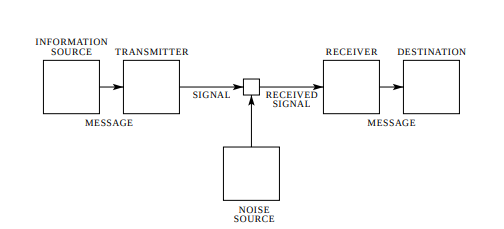
\includegraphics[width=0.65\textwidth]{comunicadorshannon.png}
  \begin{tikzpicture}
    \matrix (A) [matrix of nodes,
    column sep=25pt,
    row sep=30pt,
    nodes={minimum size=35pt}]
    {
      \node[label={[labelst]above:Fonte de\\informação},blocoq] (fonte) {}; &
      \node[label={[labelst]above:Transmissor},blocoq] (trans) {}; &
      \node[minimum size=10pt,blocoq] (conn) {}; &
      \node[label={[labelst]above:Receptor},blocoq] (rec) {}; &
      \node[label={[labelst]above:Destino},blocoq] (dest) {}; \\
      & & \node[label={[labelst]below:Fonte de \\ruído},blocoq] (ruido) {}; \\
    };
    \draw[conecta] (fonte) -- node[pos=0.5,below,labelst,yshift=-20pt] {Mensagem} (trans);
    \draw[conecta] (trans) -- node[pos=0.5,below,labelst] {Sinal} (conn);
    \draw[conecta] (conn) --  node[pos=0.5,below,labelst] {Sinal\\recebido} (rec);
    \draw[conecta] (rec) -- node[pos=0.5,below,labelst,yshift=-20pt] {Mensagem} (dest);
    \draw[conecta] (ruido) -- (conn);
  \end{tikzpicture}
  \fonte{Adaptado de \textcite[p. 380]{MTC}.}
\end{figure}

De acordo com  a TMC, um \textit{gerador de informação} é um objeto capaz de produzir um conjunto $X$ de $n$ eventos com probabilidade de ocorrência $P(X)$, enquanto um \textit{receptor} possui um conjunto $Y$, também com $n$ eventos, com probabilidades associadas $P(Y)$. Durante a transmissão é possível que parte da informação seja perdida, devido a ocorrência de ruídos, o que resulta diretamente na modificação dos valores de probabilidade dos elementos recebidos do conjunto $Y$. Reconhecendo portanto os elementos de $X$ e suas probabilidades associadas, espera-se que uma mensagem bem transmitida, ou seja, sem interferência de ruídos, seja aquela cujas probabilidades dos elementos do conjunto $Y$ sejam as mesmas dos conjunto de elementos de $X$. Assim, se essas probabilidades forem distintas, podemos concluir que houve perda de informação na transmissão \cite{mathematical}.

De maneira geral, a informação é quantificada de acordo com os recursos físicos necessários para que ela seja representada, ou seja, na capacidade de armazenamento, comunicação e representação de um conjunto $X$ de possíveis informações. Em um computador clássico, por exemplo, armazenamos informações através das unidades binárias chamadas \textit{bits}\footnote{Nome proposto, segundo o artigo original de Shannon por J.W. Turkey \cite{MTC}.}. Dessa forma, os bits são a menor unidade de armazenamento de informação em um computador de arquitetura clássica, podendo representar o estado 1 ou o estado 0 \cite{MTC}.

A combinação desses bits faz com que uma mensagem possa ser armazenada, processada ou transmitida em um computador clássico. Nesse sentido, quão maior, ou ainda, quão mais complexa for a mensagem a se operar, mais bits serão necessários e consequentemente mais recursos físicos para a representação destes.

A descrição da arquitetura de um computador quântico esbarra no mesmo princípio daquela de um computador clássico, ou seja, em sua unidade fundamental de armazenamento de informação. De maneira análoga ao computador clássico, que utiliza como unidade de informação o bit, o computador quântico utilizará o \textit{qubit} (ou q-bit, ou ainda, quantum bit).

Um qubit, ou bit quântico, pode ser produzido de maneiras distintas\footnote{Qubits podem ser fisicamente criados utilizando, por exemplo, spins de átomos presos em uma armadilha. Essa armadilha pode ser do tipo óptica ou até mesmo magnética. É possível também polarizar fótons para sua obtenção. A determinação do método é definida principalmente pelo mecanismo que melhor conseguir isolar o \textit{qubit}, já que este é facilmente influenciado pelo ambiente externo \cite{materialdidaticomecquantica}.}, porém nosso foco de estudo está nas suas propriedades. Um qubit é uma unidade com propriedades quânticas que atua sob o regime de superposição de estados. Isso significa que ele consegue armazenar simultaneamente mais de um estado de informação, diferente do bit clássico que armazena apenas um dos estados por vez. Decorre desta propriedade a maior capacidade de operar a informação em comparação aos mecanismos clássicos segundo apresentado na Tabela~\ref{tabelabit}.

\begin{table}[ht]
  \centering
  \caption{Comparação entre a quantidade de bits clássicos e quânticos necessários para se operar uma informação.}\label{tabelabit}
  \begin{tabular}{ccc}
    \toprule
    \thead{Quantidade \\ de bytes \\ (informação)} & \thead{Quantidade \\ de bits clássicos} & \thead{Quantidade \\ de qubits} \\
    \midrule
    1         & 8            & 3  \\
    \num{e6}  & \num{8.3e6}  & 23 \\
    \num{e12} & \num{8.8e12} & 43 \\
    \bottomrule
  \end{tabular}
  \fonte{Elaborada pelo autor.}
\end{table}

De modo a generalizar a comparação entre bits classicos e quânticos, podemos estabelecer a relação:
\begin{equation} \label{bitvsqubit}
n\, \text{qubits} = 2^{n}\,\text{bits}.
\end{equation}

Portanto, podemos concluir que menos qubits são necessários para operar a informação, em comparação ao bit clássico, o que está diretamente relacionado com a velocidade e com a capacidade de realização deste.

Segundo \textcite{CompInfoQuantica} e \textcite{dwave}, a devida construção de um computador de arquitetura quântica foi precedida pelos eventos descritos a seguir:

\begin{description}
  \item[1985] David Deustch propõe matematicamente o primeiro computador quântico universal;
  \item[1994] Peter Shor cria o primeiro programa essencialmente quântico, ou seja, ele não poderia ser executado em um computador clássico. Este programa, conhecido como Algoritmo de Shor, reduziria o tempo de fatoração de números grandes de possíveis meses para apenas segundos caso fosse utilizado em um computador real de arquitetura quântica;
  \item[1999] O MIT apresenta o primeiro protótipo de um computador quântico real;
  \item[2007] A empresa D-Wave apresenta o primeiro computador essencialmente quântico.
\end{description}

Apesar de na atualidade processadores quânticos existirem e operarem \footnote{FALAR SOBRE O AZURE QUANTUM E IBM QUANTUM}, ainda estamos distantes da efetiva implementação comercial de um computador quântico. Podemos utilizar de exemplo, o fato de que apesar de possuirmos um análogo para a TMC de Shannon em um computador quântico\footnote{Em 1995, Benjamin Schumacher propoẽ com êxito um análogo quântico para o TMC \cite{benschu}.}, ainda não temos um análogo quântico para um sistema submetido a ruídos na transmissão\footnote{Contudo, foi desenvolvida a teoria de correção de erros quânticos que permite que computadores quânticos possam operar na presença de ruídos e que a informação quântica seja transmitida de maneira confiável \cite{chuang}}\cite{chuang}.

Portanto, o estudo de simulações de sistemas de informação quânticos, se faz necessário para aperfeiçoamento desses mecanismos e ainda para o desenvolvimento da própria física, visto que o avanço da compreensão da utilização da mecânica quântica atrelado ao conceito de informação, possibilita a compreensão da natureza de maneira cada vez mais complexa, sem a necessidade de aproximações e simplificações \cite{chuang}.

Devido aos recursos de simulação, podemos utilizar um computador de arquitetura clássica para simular tanto um qubit quanto os circuitos lógicos necessários para a realização de operações com a informação quântica, a título do estudo, por exemplo, dos efeitos de ruídos na transmissão da informação quântica conforme propomos nesse trabalho. Nesse sentido, os próximos capítulos irão introduzir conceitos sobre informação quântica e mecânica quântica para a compreensão do desenvolvimento do trabalho.

\section{Fundamentação Teórica}

Conforme descrito no Capítulo de Introdução, para o estudo da Computação Quântica e/ou Informação Quântica, são necessários alguns recursos provenientes da Mecânica Quântica bem como a construção de análogos quânticos para o processamento dessa informação. As Seções a seguir apresentarão a fundamentação teórica e os recursos matemáticos necessários para o desenvolvimento da simulação proposta na Metodologia.

\subsection{Conceitos básicos de Álgebra Linear}


\subsection{Mecânica Quântica}\label{Mecanicaquantica}

Esta teoria foi criada no início do século XX para explicar o comportamento dos átomos e estudar os efeitos relativos ao tamanho microscópico das partículas. A mecânica quântica explica como as partículas subatômicas se comportam, como interagem com a luz e como são afetadas por forças externas. Esta teoria é usada para explicar muitos fenômenos físicos, como a estrutura de átomos e moléculas, a propriedades de materiais, a propriedades de radiação eletromagnética, e a propriedades de matéria escura.
Podemos definir seus postulados como:
\begin{enumerate}
\item Princípio da incerteza de Heisenberg: é impossível, ao mesmo tempo, medir com precisão a localização e a velocidade de uma partícula subatômica.

\item Princípio da dualidade onda-partícula: uma partícula subatômica pode se comportar tanto como onda quanto como partícula.

\item Princípio da superposição: qualquer sistema quântico pode encontrar-se simultaneamente em vários estados.

\item Princípio da exclusão de Pauli: dois fótons ou partículas idênticas não podem ocupar o mesmo estado quântico.

\item Princípio da ação à distância: o efeito de uma interação quântica entre partículas pode se propagar instantaneamente, independentemente da distância.
\end{enumerate}

Para os estudos que seguem nesse trabalho, iremos enfatizar os postulados 3 e 5.


\subsection{Qubits}
Definição

As definições de qubits descritas nesse tópico, baseiam se principalmente nas idéias apresentadas por \textcite{chuang} e \textcite{CompInfoQuantica}.

Qubits são elementos fundamentais da computação quântica. Eles são usados para representar informações binárias (zeros e uns) e são capazes de armazenar e processar muito mais informações que os bits convencionais usados na computação clássica. Isso é possível graças ao fato de que, enquanto os bits tradicionais podem estar em dois estados (ligado ou desligado), os qubits podem estar em um estado de superposição, que permite que eles representem simultaneamente vários estados ou informações diferentes.Isso significa que os qubits podem armazenar muito mais informações em um espaço muito menor, tornando a computação quântica muito mais poderosa e eficiente.

Podemos começar a descrição de um qubit como uma superposição dos estados quânticos $\ket{0}$ e $\ket{1}$, de modo que podemos representá-los pela combinação linear dada por:

\begin{equation}\label{psi}
\ket{\psi} = \alpha \ket{0} + \beta \ket{1} \quad \text{com $\alpha$ e $\beta$ parametrizados por} \quad \alpha^{2} + \beta^{2} = 1
\end{equation}

Os números $\alpha$ e $\beta$ são complexos e determinam as amplitudes probabilisticas da obtenção dos estados quânticos.
O estado descrito por $\ket{\psi}$ é uma superposição dos estados quânticos $\ket{0}$ e $\ket{1}$, ou seja, seguindo os postulados da mecânica quântica, o qubit pode existir num estado contínuo entre $\ket{0}$ e $\ket{1}$ porém, ao ser medido, colapsando o sistema, retornará apenas os valores de $\ket{0}$ e $\ket{1}$ com as probabilidades $\alpha$ e $\beta$ associadas.

Um recurso para visualizar o comportamento de qubits é sua representação geométrica chamada de Esfera de Boch. Como entidades quânticas não são observáveis diretamente e frequentemente expressas por recursos matemáticos, a visualização da superposição dos estados de um qubit utilizando a Esfera de Boch facilita, ligeiramente, sua compreensão.
Em primeiro lugar, vale lembrar que o qubit, descrito por $\ket{\psi}$ está parametrizado e podemos reescrever \ref{psi} em coordenadas polares de modo que:

\begin{equation}
\ket{\psi}=e^{i \gamma}\left(\cos \frac{\theta}{2}\ket{0}+e^{i \varphi} \sin \frac{\theta}{2}\ket{1}\right)
\end{equation}

A primeira parte da equação não possui efeitos observáveis na representação geométrica e portanto, podemos simplificar a equação acima como:

\begin{equation}
\ket{\psi}=\left(\cos \frac{\theta}{2}\ket{0}+e^{i \varphi} \sin \frac{\theta}{2}\ket{1}\right),
\end{equation}
com $\theta$ e $\varphi$ sendo números reais correspondentes aos ângulos entre os eixos $z$, $y$ e $y$,$x$ respectivamente conforme Fig. \ref{boch}

\begin{figure}[ht!]
\centering
\caption{Representação gŕáfica de um qubit como um ponto sob a superfície da Esfera de Boch}\label{boch}
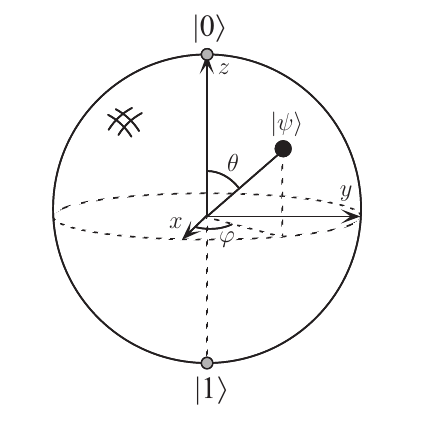
\includegraphics[width=10cm]{boch.png}
\fonte{Adaptado de \cite{chuang}}
\end{figure}

%EXPLICAR COMO FUNCIONA O ARMAZENAMENTO DE INFORMAÇÃO NO QUBIT E COMO FUNCIONA A MEDIDA DE UM ESTADO

\subsection{Portas Lógicas Quânticas}

%As portas lógicas quânticas são operadores quânticos usados para construir circuitos quânticos. Elas são usadas para manipular e controlar a informação codificada em qubits. As portas lógicas quânticas são fundamentais para a computação quântica, pois são usadas para realizar operações lógicas e computacionais. Existem diversos tipos de portas lógicas quânticas, incluindo portas NOT, portas XOR, portas AND, portas OR, portas CNOT, portas SWAP e outras. Cada porta quântica tem sua própria função e é usada para realizar operações lógicas e computacionais.
%
%Porta Lógica CNOT Quântica
%
%A Porta Lógica CNOT Quântica é usada para implementar operações condicionais e permutações entre qubits. Ela é usada para criar circuitos lógicos quânticos mais complexos. Esta porta é uma versão geral da porta CNOT clássica, pois ela pode ser aplicada a todos os qubits, não apenas dois. Na porta CNOT quântica, o qubit de controle é usado para controlar o estado de outro qubit (alvo). Se o qubit de controle estiver em 1, o estado do qubit alvo será invertido, mas se o qubit de controle estiver em 0, o estado do qubit alvo não será alterado. A porta CNOT quântica também pode ser usada para realizar permutações, ou seja, trocar o estado de dois qubits.
%
%
%Porta Lógica Hadamard Quântica
%
%
%A Porta Lógica Hadamard Quântica (HQ) é uma porta lógica quântica que transforma o estado de um qubit (quântico bit) em seu estado oposto com 50\% de probabilidade. Ela pode ser usada para realizar operações de entrelaçamento entre qubits, o que permite a implementação de algoritmos quânticos complexos. A porta HQ foi desenvolvida com o objetivo de permitir o controle preciso de qubits em circuitos quânticos. Ela é representada por um matrix unitário de 2x2, que é definido como: 
%
%[1/√2, 1/√2]
%[1/√2, -1/√2]
%
%Onde √2 é a raiz quadrada de dois. A funcionalidade da porta HQ é a de transformar o estado de um qubit de 0 para 1 ou de 1 para 0. A porta HQ pode ser usada para criar entrelaçamentos entre qubits, o que permite a implementação de algoritmos quânticos complexos. A porta HQ pode ser usada para implementar muitos algoritmos quânticos, como o algoritmo de Grover, o algoritmo de Shor e o algoritmo de Adiabat. Além disso, a porta HQ pode ser usada para implementar circuitos quânticos, como o circuito de computação quântica.


\subsection{Emaranhamento Quântico}

%O emaranhamento quântico é o fenômeno pelo qual partículas elementares, como fótons, elétrons e outras, ligam-se entre si de tal maneira que um objeto passa a ter quase que uma única identidade. Neste estado, um objeto passa a ter propriedades que estão além dos limites da mecânica quântica. Em outras palavras, o emaranhamento quântico é um estado no qual duas partículas interagem de forma tal que elas compartilham o mesmo estado e não podem ser descritas independentemente. Por exemplo, dois fótons entrelaçados podem ser entendidos como uma única partícula, mesmo que eles estejam distantes um do outro. O emaranhamento quântico pode ser usado para criar ligações entre partículas e objetos distantes, o que abre portas para o desenvolvimento de novas tecnologias, como a computação quântica.
%
%Etapas do Emaranhamento Quântico de Qubits
%
%\begin{itemize}
%\item 1. Preparação:  O primeiro passo é preparar os qubits individuais. Isso pode ser feito carregando os qubits em computadores quânticos ou usando dispositivos quânticos especializados, como lasers.
%
%\item 2. Entrelaçamento: Em seguida, os qubits são entrelaçados, o que significa que eles são interconectados de modo que as informações entre eles sejam compartilhadas. Isso pode ser feito usando técnicas como a interferência quântica.
%
%\item 3. Operações: Uma vez que os qubits estão entrelaçados, as operações quânticas podem ser realizadas neles. As operações podem incluir a realização de computações quânticas complexas, o armazenamento de informações quânticas ou o envio de informações entre qubits.
%
%\item 4.Saída: Por fim, os qubits podem ser desentrelaçados para obter a saída desejada. Isso pode ser feito usando técnicas como a interferência quântica inversa. A saída pode incluir informações codificadas nos qubits, como um resultado de uma computação quântica.
%
%\end{itemize}



\subsection{Teletransporte Quântico}
%O  Teletransporte Quântico 
%
%O Teletransporte Quântico é um processo de transferência de informação quântica entre dois pontos, usando mecanismos quânticos. Essa transferência pode ocorrer quase instantaneamente, independentemente da distância entre os dois pontos.
%O Teletransporte Quântico é baseado em princípios da mecânica quântica, que descrevem como os estados quânticos podem ser compartilhados entre partículas e aplicados aos sistemas de informação. O Teletransporte Quântico foi descoberto pela primeira vez pela física austríaca Anton Zeilinger, em 1998. Ela escobriu que, usando um fenômeno conhecido como entrelaçamento quântico, é possível transferir informação instantaneamente entre dois pontos. O princípio básico do teletransporte quântico é que dois partículas, como elétrons, átomos ou fótons, podem ser entrelaçados, ou ligados entre si. Quando isso acontece, qualquer mudança na configuração de uma partícula será imediatamente refletida na outra, mesmo que elas estejam separadas por uma distância enorme. Isso significa que informação pode ser enviada instantaneamente entre dois pontos distantes.
%
%Embora o teletransporte quântico ainda esteja em fase experimental, já foi usado para transferir informações básicas como posição, polarização e estado de spin entre dois pontos separados. A tecnologia ainda precisa desenvolver muito antes de poder ser usada para transferir informações mais complexas, como imagens ou dados.
%
%Na prática, o Teletransporte Quântico permite que um estado quântico seja transferido de um lugar para outro, sem que nenhuma informação seja transferida entre os locais. Isso significa que um estado quântico pode ser transmitido de uma parte do universo para outra sem que nenhuma informação seja trocada entre eles.
%O Teletransporte Quântico é usado em diversas áreas científicas, como criptografia, computação quântica, comunicação segura e muito mais. Também pode ser usado para transferir informações confidenciais de um lugar para outro, impedindo que terceiros interceptem a informação.


\subsection{Protocolo de Teletransporte Quântico}

A realização de um Protocolo de Teletransporte Quântico consiste, essencialmente, em uma série de operações que possuem por objetivo principal fazer com que uma mensagem, ou na linguaguem quântica, um estado quântico se teletransporte entre dois pontos distintos fisicamente. 
Como em qualquer outra operação computacional é necessária a existencia de um circuito lógico, nesse caso, quântico que media as operações. Esse circuito consistirá nas combinações das portas lógicas CNOT, Haddamard, portas de medição e as portas X e Z conforme Figura \ref{protocoloteletransporte}
-

\begin{figure}
\centering
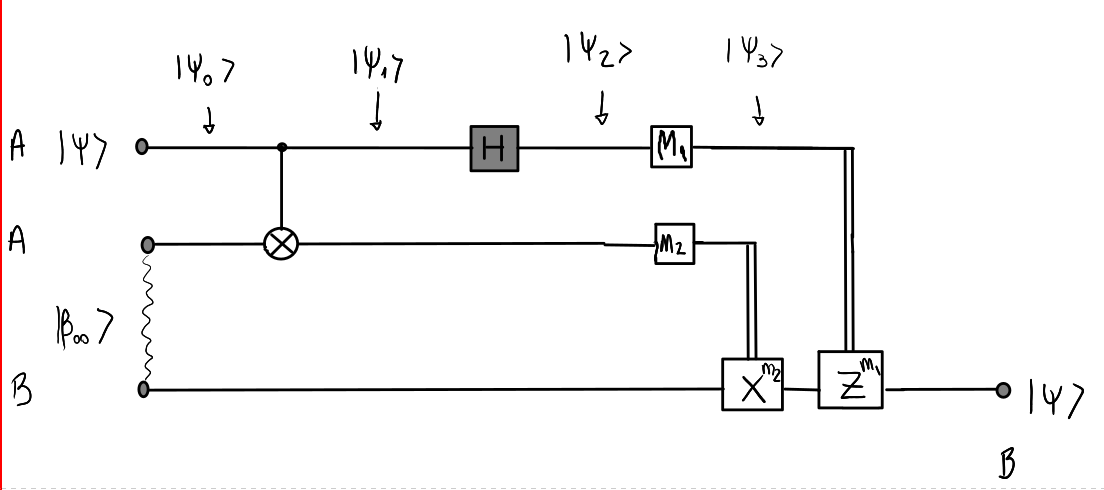
\includegraphics[width=10cm]{PROTOCOLOTELETRANSPORTE.png}
\caption{Protocolo de Teletransporte Quântico mediado pelo circuito com as portas CNOT, Hadamard, Medição aplicadas no Local A e as portas X e Z aplicadas no Local B.}\label{protocoloteletransporte}
\fonte{Adaptado de }
\end{figure}

No inicio do Protocolo é necessário, que tenhamos um par de qubits emaranhados nas bases de Bell, no estado $\ket{\beta_{00}}$, que podemos representar pela expressão:

\begin{equation}\label{bell00}
 \ket{\beta_{00}} = \frac{\ket{00} + \ket{11}} {\sqrt{2}}.
\end{equation}

Um dos qubits do par emaranhado em \ref{bell00} é mantido em A e o outro necessáriamente precisa estar em B para que exista um canal de comunicação entre essas partes. Além do par emaranhado, em A teremos o estado quântico a ser enviado, ou seja sua mensagem dada por $\ket{\psi}$, segundo:

\begin{equation}\label{psi}
 \ket{\psi} = \alpha \ket{0} + \beta \ket{1}.
\end{equation}

De posse do par emaranhado e da mensagem, o protocolo é iniciado com a aplicação da porta CNOT entre $\ket{\psi}\ket{\beta_00}$, que chamaremos de $\ket{\psi_0}$. A porta CNOT possui como tabela verdade a seguinte proposição:

\begin{theo}{Operação CNOT}{cnottheo}
A operação CNOT deve: i.Inverter o segundo qubit, caso o primeiro esteja no estado $\ket{1}$; ii. Não realizar nenhuma operação no segundo qubit, caso o primeiro esteja no estado $\ket{0}$.
\end{theo}

Dessa maneira, aplicando ~\ref{cnottheo} no estado dado por $\ket{\psi_0}$

\begin{eqnarray}\label{cnotpsi0}
CNOT \ket{\psi_0} = CNOT \ket{\psi} \ket{\beta_{00}} = \nonumber \\ 
CNOT \frac{1}{\sqrt{2}} \left[ \alpha  \ket{0} \left( \ket{00} + \ket{11} \right) + \beta \ket{1} \left( \ket{00} + \ket{11} \right)\right] = \nonumber \\
\frac{1}{\sqrt{2}} \left[\alpha \ket{0} \left( \ket{00} + \ket{11} \right) + \beta \ket{1} \left( \ket{10} + \ket{01} \right) \right].
\end{eqnarray}

A operação descrita em \ref{cnotpsi0} resulta no estado que chamaremos de $\ket{\psi_1}$ e neste, segundo o circuito \ref{protocoloteletransporte}, deve-se aplicar a porta Hadamard:

\begin{theo}{Operação Hadamard}{hadamardtheo}
A operação Hadamard deve: Aplicar no estado 0 a operação $\frac{1}{\sqrt{2}} \left(\ket{0}+\ket{1}\right)$; Aplicar no estado 1 a operação $\frac{1}{\sqrt{2}}\left(\ket{0}-\ket{1}\right)$.
\end{theo}

Aplicando portanto o ~\ref{hadamardtheo} em $\ket{\psi_1}$, teremos:

\begin{equation}\label{hadamartpsi2}
 H \ket{\psi_1} = \left( \frac{1}{\sqrt{2}}\right)^{2} \left[ \alpha \left( \ket{0} + \ket{1} \right)\left( \ket{00} +\ket{11} \right)+ \beta \left( \ket{0} - \ket{1} \right) \left( \ket{10} + \ket{01} \right) \right].
\end{equation}

O estado obtido em \ref{hadamartpsi2} pode ser identificado como $\ket{\psi_2}$ e 
evidenciando os estados emaranhados deste organizando-o da seguinte maneira:

\begin{equation}\label{psi2}
 \ket{\psi_2} = \frac{1}{2} \left[ \ket{00} ( \alpha \ket{0} + \beta \ket{1} ) + \ket{01} ( \alpha \ket{1} + \beta \ket{0} ) + \ket{10} ( \alpha \ket{0} - \beta \ket{1} ) + \ket{11} ( \alpha \ket{1} - \beta \ket{0} ) \right].
\end{equation}

O próximo passo do protocolo consiste em realizar medidas em ambos os qubits presentes em A. Essas medidas, farão com que o estados quânticos dos mesmos sejam colapsados e deixem de coexistir, passando a ser considerados clássicos. As medidas possíveis de serem obtidas em A são:

\begin{table}[ht!]
\centering
\caption{Possíveis resultados das medidas realizadas nos qubits presentes em A no estado quântico $\ket{psi_2}$.}\label{medidas}
\begin{tabular}{cc}
 {Medida realizada} & {Estado quântico associado}\\
 \hline
 $\ket{00}$   & $\left( \alpha \ket{0} + \beta \ket{1} \right)$\\
 $\ket{01}$   & $\left( \alpha \ket{1} + \beta \ket{0} \right)$\\
 $\ket{10}$   & $\left( \alpha \ket{0} - \beta \ket{1} \right)$\\
 $\ket{11}$   & $\left( \alpha \ket{1} - \beta \ket{0} \right)$

  \end{tabular}
  \fonte{Elaborada pelo autor.}
\end{table}

Os valores dos estados medidos em A, são enviados via canal clássico até B que, devido ao emaranhamento com o qubit operado em A, terá seu colapso consequentemente em seu estado quântico associado, segundo tabela \ref{medidas}.

A última etapa do protocolo, ocorre em B, na tentativa de reconstruir a mensagem original, nesse momento já inexistente, que estava em A. Nessa última etapa, serão utilizadas (ou não) as portas lógicas X e Z cujas operações são definidas por:

\begin{theo}{Operação X}{X}
A porta lógica quântica X deve trocar os estados quânticos, ou seja, torná-lo 1 quando este for 0 e torná-lo 0, quando este for 1.
\end{theo}

\begin{theo}{Operação Z}{Z}
A porta lógica quântica Z deve inverter a fase do estado quântico, ou seja, torná-la negativa quando esta for positiva e torná-la positiva quando esta for negativa.
\end{theo}

A aplicação das portas, dependerá do resultado da medida enviado por A de maneira que:

\begin{itemize}
\item Se a medida for $\ket{00}$: Nenhuma porta deve ser aplicada e o estado colapsado em B é exatamente o mesmo da mensagem enviada em $\ket{psi}$.
\item Se a medida for $\ket{10}$: Apenas a porta Z deve ser aplicada.
\item Se a medida for $\ket{01}$: Apenas a porta X deve ser aplicada.
\item Se a medida for $\ket{11}$: Tanto a porta X quanto a porta Z devem ser aplicadas.
\end{itemize}

Com isso, o protocolo se encerra e a mensagem é teletransportada do ponto A para o ponto B, sem que nenhum teorema da física quântica seja violado.


\subsection{Algoritmo do protocolo de Teletransporte}

Descrição das etapas para o protocolo de teletransporte

\begin{enumerate}
\item Determinar as funções que descrevem os qbits a serem emaranhados
	\begin{itemize}
	\item qbit x
	\item qbit y
	\end{itemize}
\item Determinas as matrizes que descrevem as portas utilizadas no emaranhamento
	\begin{itemize}
	\item Porta Hadamard
	\item Porta CNOT
	\item Matriz Identidade
	\end{itemize}
\item Determinar as operações entre os qbits e as portas e a ordem de realização para o emaranhamento
	\begin{itemize}
	\item Produto tensorial entre qbit x e qbit y $\rightarrow$ qbit xy
	\item Produto tensonial entre Porta Haddamard e Matriz Identidade $\rightarrow$ H $\otimes$ I
	\item Multiplicação entre qbit xy e H $\otimes$ I $\rightarrow$ Hxy
	\item Multiplicação entre Hxy e a Porta CNOT $\rightarrow$ $\beta _00$
	\end{itemize}
\item Determinar o qbit a ser enviado
	\begin{itemize}
	\item Definir a entrada de dados feita pelo usuário
	\item Verificar a possibilidade de acordo com a normalização $\alpha + \beta =1$
	\end{itemize}
\item Aplicar a porta CNOT
	\begin{itemize}
	\item Verificar a condição lógica de aplicação da porta CNOT
	\item Aplicar CNOT em $\beta _00$ $\rightarrow$ $\ket{\psi _1}$
	\end{itemize}
\item Aplicar a porta Hadamard em $\ket{\psi _1}$ $\rightarrow$ $\ket{\psi _2}$
\item Reorganizar e apresentar os estados antes da medição
\item Realizar a medição
	\begin{itemize}
	\item Determinar de modo aleatório qual dos estados serão medidos
	\end{itemize}
\item Apresentar a medição - Transmissão clássica da informação
\item Determinar as operações a serem realizadas de acordo com a medição realizada
\item Apresentar a mensagem original recuperada	
\end{enumerate}

\subsection{Ruídos}
%Os ruídos no teletransporte de informação quântica são aqueles que se produzem durante o processo de transferência de dados quânticos entre dois sistemas distintos. Esses ruídos podem ser de natureza física ou de natureza lógica.
%
%Ruídos físicos são aqueles que se originam de fontes externas, como ruídos elétricos, ruídos electromagnéticos e ruídos térmicos, entre outros. Esses ruídos incluem:
%\begin{itemize}
%\item 1. Interferência de radiação: a radiação eletromagnética proveniente de fontes externas, como estações de rádio e antenas, pode interferir no sinal quântico, distorcendo ou desviando-o de seu destino.
%
%\item 2. Perda de informação: devido às fracas interações entre os componentes da rede quântica, parte da informação pode ser perdida ao longo do caminho, afetando a qualidade e a confiabilidade da transferência.
%
%\item 3. Decoerência: é o fenômeno quântico que pode ocorrer ao longo do caminho, onde a entropia ou o desordem de um sistema aumentam, o que pode levar a erros na recepção de informações.
%
%\item 4. Entropia térmica: o calor presente no ambiente pode levar a alterações nos estados quânticos dos componentes da rede, o que pode levar a erros na transferência de informações.
%
%\item 5. Interferência mecânica: as vibrações e os ruídos mecânicos presentes no local de transferência de informações podem afetar a qualidade e a confiabilidade dos dados transferidos.
%\end{itemize}
%
%Ruídos lógicos são aqueles que surgem a partir do processo de transferência de dados quânticos, como erros de codificação, erros de decodificação e erros de sincronização. Podemos ressaltar:
%\begin{itemize}
%\item 1. Falha na sincronização de tempo: a sincronização de tempo é um passo crítico para o teletransporte quântico. Se os relógios entre os dois locais não estiverem sincronizados, o teletransporte pode falhar.
%
%\item 2. Desequilíbrio de energia: o desequilíbrio de energia pode ocorrer devido aos efeitos de decaimento quântico, o que pode causar a falha do teletransporte.
%
%\item 3. Interferência de campo: o campo de força entre os dois locais pode interferir com os processos quânticos necessários para o teletransporte.
%
%\item 4. Erro de medição: a medição incorreta dos estados quânticos dos dois locais pode resultar em erros que resultam na falha do teletransporte.
%
%\item 5. Vazamento de informação: o vazamento de informação pode levar à perda de informação necessária para o teletransporte quântico.
%\end{itemize}
%
%Além disso, existem também ruídos de medição, que são aqueles que surgem durante as medições quânticas, e ruídos de decoerência, que são aqueles que se produzem durante a decoerência do estado quântico.
%
%Para minimizar os efeitos dos ruídos no teletransporte de informação quântica, é importante realizar a otimização dos protocolos de teletransporte, otimizar o processo de codificação e decodificação e utilizar técnicas de processamento de sinal quântico.

\section{Metodologia}

\section{APÊNDICE}

\subsection{Representação Matricial dos protocolos e Emaranhamento e Teletransporte}

As representações matriciais dos protocolos de Emaranhamento e Teletransporte nos permitem observer com maior clareza a natureza binária dos qubits numa representação de como seria seu comportamento em uma situação real. Para todos os efeitos não é considerada a origem do qubit mas sim sua natureza, ou seja, uma entidade quântica. A notação de bracket permite com que as operações sejam realizadas considerando os estados quânticos possíveis armazenados dentro do qubit como versores num espaço complexo.
Para iniciar o protocolo, consideraremos as seguintes representações binárias dos estados quânticos:

\begin{equation} \label{01}
\ket{0} = \left(\begin{array}{l}
0 \\
1
\end{array}\right) \; e \;
\ket{1} = \left(\begin{array}{l}
1 \\
0
\end{array}\right)
\end{equation}

Consideraremos também que estados quânticos que dependem de mais de um qubit (emaranhados ou não), são representados pelo produto tensorial dos seus estados internos, como segue o exemplo:

\begin{equation}\label{00}
\ket{00} = \left(\begin{array}{l}
0 \\
1
\end{array}\right) \otimes \left(\begin{array}{l}
0 \\
1
\end{array}\right) = \left(\begin{array}{l}
1 \\
0 \\
0 \\
0
\end{array}\right)
\end{equation}

A representação gráfica do circuito quântico que realiza o protocolo de emaranhamento possibilita o entendimento dos procedimentos contidos no mesmo, conforme Fig \ref{circuitoemr}

INSERIR FIGURA CIRCUITO EMARANHAMENTO

Para que o emaranhamento seja possível, ambos os qubits representados por $\ket{q_x}$ e $\ket{q_y}$ devem existir no mesmo espaço de Hilbert e portanto a operação de produto tensorial entre eles deve ser possível de modo que, considerando o estado quântico $\ket{0}$:

\begin{equation}
\ket{q_x} \otimes \ket{q_y} = \ket{0} \otimes \ket{0} = \ket{00} = \left(\begin{array}{l}
0 \\
1
\end{array}\right) \otimes \left(\begin{array}{l}
0 \\
1
\end{array}\right) = \left(\begin{array}{l}
1 \\
0 \\
0 \\
0
\end{array}\right)
\end{equation}

Seguindo a figura, aplicamos a porta Hadamard H na Eq., multiplicando a mesma pela matriz identidade I, obtendo:

\begin{equation}
H \otimes I = 1/\sqrt{2} \left(\begin{array}{l}
1 1 \\
1 -1 
\end{array}\right) \otimes \left(\begin{array}{l}
1 0 \\
0 1
\end{array}\right) = 1/\sqrt{2} \left(\begin{array}{l}
\begin{matrix}
1 & 0 & 1 & 0 \\
0 & 1 & 0 & 1 \\
1 & 0 & -1 & 0 \\
0 & 1 & 0 & -1
\end{matrix}
\end{array}\right)
\end{equation}

e, aplicando o resultado acima em \ref{00}:

\begin{equation}
H \ket{00} = 1/\sqrt{2} \left(\begin{array}{l}
\begin{matrix}
1 & 0 & 1 & 0 \\
0 & 1 & 0 & 1 \\
1 & 0 & -1 & 0 \\
0 & 1 & 0 & -1
\end{matrix}
\end{array}\right) \left(\begin{array}{l}
1 \\
0 \\
0 \\
0
\end{array}\right) = 1/\sqrt{2} \left(\begin{array}{l}
1 \\
0 \\
1 \\
0
\end{array}\right)
\end{equation}

Em seguida, aplicamos a porta CNOT:

\begin{equation}
\left(\begin{array}{l}
\begin{matrix}
1 & 0 & 0 & 0 \\
0 & 1 & 0 & 0 \\
0 & 0 & 0 & 1 \\
0 & 1 & 1 & 0
\end{matrix}
\end{array}\right) 
1/\sqrt{2}\left(\begin{array}{l}
1 \\
0 \\
1 \\
0
\end{array}\right) = 1/\sqrt{2} \left(\begin{array}{l}
1 \\
0 \\
0 \\
1
\end{array}\right)
\end{equation}


A equação também é conhecida por ser uma das Bases de Bell. A comparação da Base de Bell no estado $\ket{00}$ em notação de Dirac e em notação matricial é dada por:

\begin{equation}
\text{Seja} \ket{\beta_00} \text{a Base de Bell em notação de Dirac dada por:} 1/\sqrt{2} (\ket{00} + \ket{11}), \text{reescrevendo teremos:}
\end{equation}
% FALTA TERMINAAAAAAAR!
%




\clearpage
\printbibliography[heading=subbibliography]

\end{document}